% Please do not change the document class
\documentclass{scrartcl}

% Please do not change these packages
\usepackage[hidelinks]{hyperref}
\usepackage[none]{hyphenat}
\usepackage{setspace}
\doublespace

% You may add additional packages here
\usepackage{amsmath}
\usepackage{graphicx} 
\graphicspath{ {Diagrams/} }

% Please include a clear, concise, and descriptive title
\title{ Companion AI using a Behaviour Tree }

% Please do not change the subtitle
\subtitle{COMP230 - Game Component}

% Please put your student number in the author field
\author{1507866}

\begin{document}
	
\maketitle
	
\section{Outline}
My component is a companion animal AI using a behaviour tree in C++. My prototype is based on a Falcon therefore some of the branches are specific to a falcon but can easily be changed. The AI will have a series of branches that correspond to sets of behaviours such as searching  for useful objects for the player, searching for enemies, attacking/stunning them and fleeing when injured.  The branch changes are triggered when the current branches fails or succeeds.

Figure 1 shows the initial layout of the branches.  

\begin{figure}[h]
	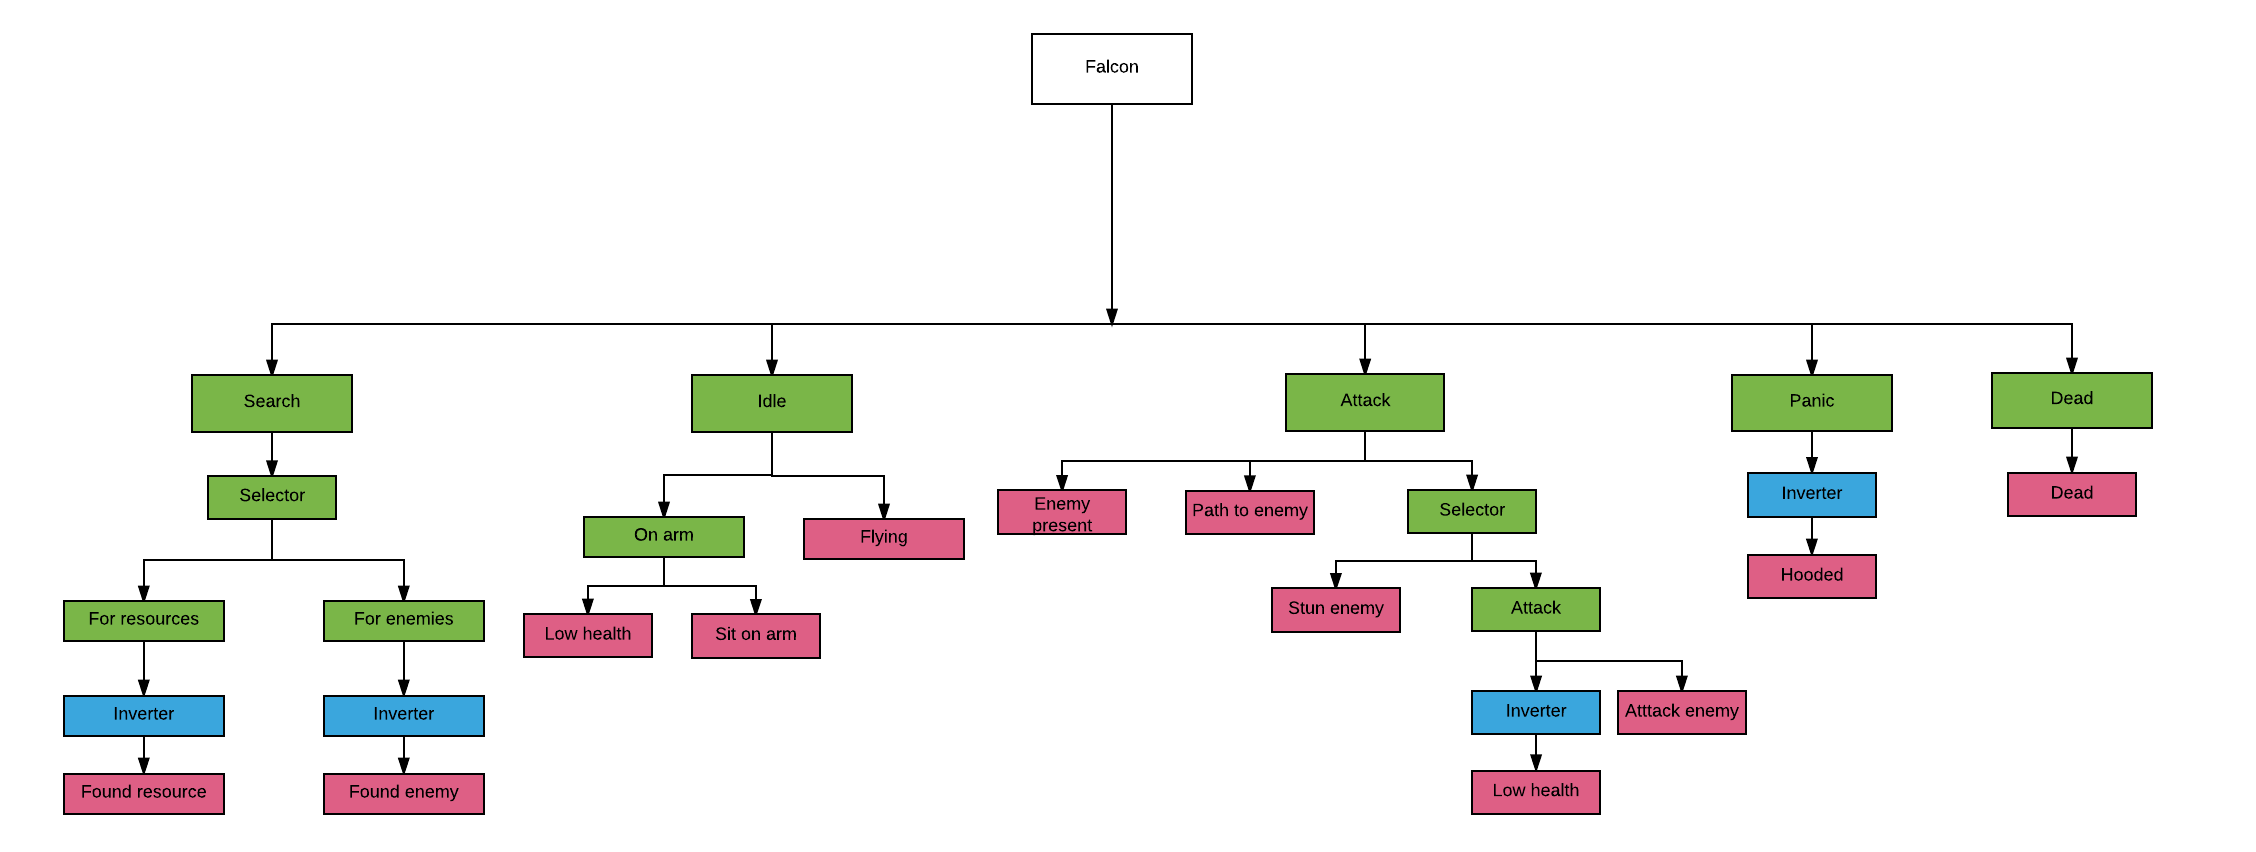
\includegraphics[width=1.2\linewidth]{behaviour_tree.png}
	\caption{ Behaviour tree being used on a falcon companion}
\end{figure} 

In figure 1 green represents sequence nodes, yellow is for selector nodes, blue for decorator and pink for leaf nodes.
 
\newpage

\section{Market Research}
Birds do not appear in games very often, they are mostly used as part of the environment that flies off when the player enter an area. Or sometimes as the playable character in games such as Eagle Flight and How We Soar. 
When researching companion AIs I found that they are often human \cite{DragonAge, LastOfUs, Bioshock}. There are also a number of features/behaviours that players say are required for a good AI companion. 
\bigskip
Two popular companions are Ellie from The Last of Us and Elizabeth from Bioshock Infinite. Both AIs aid the player by fetching helpful in game items, assisting in battles and leading the player towards the next goal in the game.
Guiding the player is a common behaviour in AI. I decided to use these three keys behaviours in my AI; the falcon will guide the player using paths generated by the terrain generator, aid the player by finding useful objects and assist the player in battles by stunning or attacking enemies and fleeing when its health is low.



\section{Scope and Commercial Feasibility}
The scope of the component depends on the number of branches implemented. Once the nodes are working it's relatively easy to adapt and add branches.

There are numerous behaviour tree tools on the Unity Asset store. The price of these tools varies from being free to \pounds225. Most of the tools come with a GUI so mine would need to be significantly cheaper as it is likely more difficult to use.
The Unity Asset store guidelines say that packages priced over \$50 are often the best selling ones. Also when looking at behaviour tree tools on the Asset store many of the best selling tools are above that price. This suggests that somewhere around \$50 would be a good price for my tool if I added a GUI to make it more accessible to users.  A potential issue with using a platform such as the Unity Asset store is that the store will take a cut of the money made from it.
The target audience is indie game developers with little code experience or developers trying to make a quick prototype.
\bigskip

A unique selling point is that most behaviour trees tools on the asset store are general tools not specific to companion AIs mine is specifically designed for companions. 


\section{ Working with PCG Navigable Terrain Component }
The PCG of the terrain itself does not effect my AI as it's currently a flying bird. However the terrain generated will use pathfinding to find navigable terrain for the player. These paths will be shared with the AI allowing it  to direct the player in the desired direction. 

\bibliographystyle{ieeetr}
\bibliography{comp230}
	
\end{document}
